\section{Test Approach}
\label{sec:test_stra}

This section describes the tests execution model, techniques and types of tests to be executed during openETCS tool chain development life cycle.

\subsection{Tests Execution Model}
The openETCS tool chain development is divided into  fortnightly sprints, on which objectives are defined and tasks that meet the requirements specified by the other workpackages and/or project goals and needs at that time (sprint) are analyzed, planned and developed. Each sprint is taken as a project in itself with their schedules, tracking daily meetings, etc.

In each iteration the scrum team evolves the product (makes an incremental delivery) from the results completed in previous iterations, adding new objectives / requirements or improving those that have already been completed. A key to guide the iterative and incremental development is the prioritization of objectives / requirements depending on the value provided to the openETCS partnes and workpackages.

In the quality control stage of each sprint, unit testing, integration testing, performance, functional and acceptance testing will be made in the test environments ensuring the quality of the openETCS tool chain.

\begin{figure}[htbp]
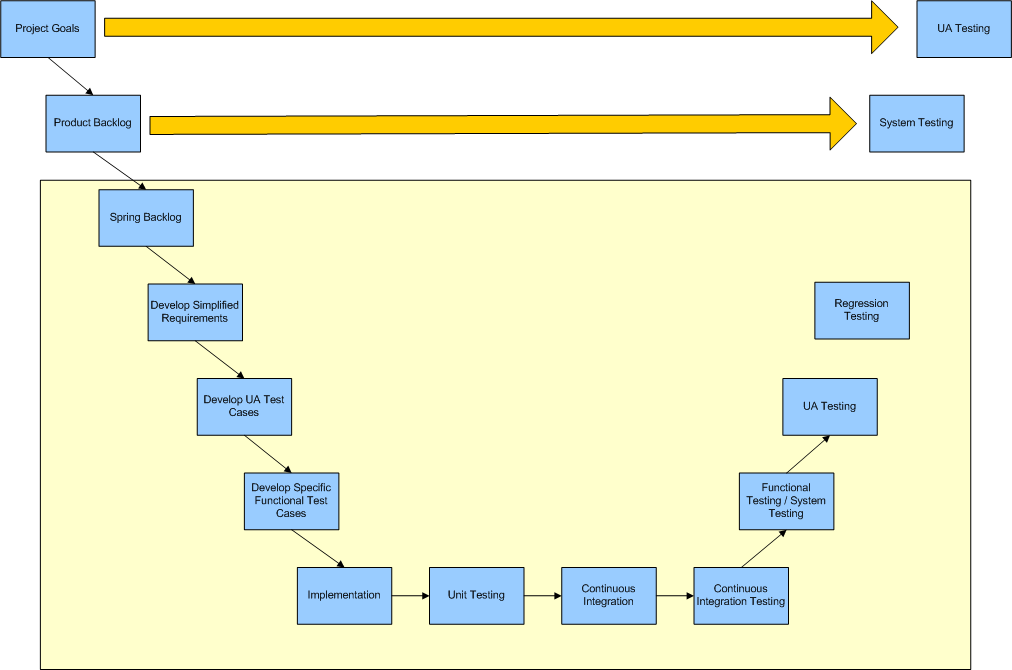
\includegraphics[width=\textwidth]{types_test}
\caption{\label{fig:types} Types of test during the development life cycle} 
\end{figure}


The fact of rerun every test every sprint it is time consuming so in each sprint unit testing will be executed continuosly and a good regression set based on risk classifications and business value will be collected and executed to give more time to specify and execute test cases for the functionalities implemented during the current sprint. All cross-sections along the subsets of test cases can form the total regression tests that are selected.

If the toolchain reach the stage of functional testing with too critical and / or blocking errors the tool chain will be returned to the unit testing stage

\subsection{Tests Types}
The validation has to demonstrate that the openETCS tool chain covers all the requirements and features.

At following the type of tests to be executed will be described.

\begin{center}
\begin{longtable}[H]{|p{4cm}|p{9cm}|}\hline
\multicolumn{2}{|c|}{\textbf{Unit Tests}}\\\hline
\textbf{Objective} &  Test the separate pluggings, or independent software areas.\\\hline
\textbf{Method} & \\\hline
\textbf{Tools} & JUnit, part of Jenkins\\\hline
\textbf{Responsible} & Product Developer\\\hline
\textbf{Execution Type} & Automatic\\\hline
\textbf{Timing} & Continuosly \\\hline
\textbf{Evaluation criteria / Exit Criteria} & \begin{itemize}
\item 100\% Test Scripts executed
\item 97\% pass rate of Test Scripts
\item No open Critical and high severity defects
\item 97\% of medium severity defects have been closed 
\item All remaining defects have been managed
\item 100\% code coverage
\item the reports generated by the test automation tools contains the minimum variables to allow a proper analysis of the evidence
\end{itemize} \\\hline
\end{longtable}
\end{center}

\begin{center}
\begin{longtable}[H]{|p{4cm}|p{9cm}|}\hline
\multicolumn{2}{|c|}{\textbf{Integration Tests}}\\\hline
\textbf{Objective} &  Validate that the OpenETCS platform and the pluggings are correctly installed, and their interoperability is correctly working. Validate the integration between different modules / plugins that make up the tool chain in order to ensure their integrated operation is correct.\\\hline
\textbf{Method} & Botton–up strategy \\\hline
\textbf{Tools} & Maven\\\hline
\textbf{Responsible} & Validation and Verification Team\\\hline
\textbf{Execution Type} & Automatic and manual\\\hline
\textbf{Timing} & \begin{itemize}
\item Automatic tests: Continuosly
\item Manual tests: only on official releases (every 6 months). For each release, a new column will be added to the table toolchain/tool/tests
\end{itemize}  \\\hline
\textbf{Evaluation criteria / Exit Criteria} & \begin{itemize}
\item 100\% Test Scripts executed
\item 97\% pass rate of Test Scripts
\item No open Critical and high severity defects
\item 97\% of medium severity defects have been closed 
\item All remaining defects have been managed
\item The total coverage of the tested is greater than 80\% of all modules
\end{itemize} \\\hline
\end{longtable}
\end{center}

\begin{center}
\begin{longtable}[H]{|p{4cm}|p{9cm}|}\hline
\multicolumn{2}{|c|}{\textbf{System Tests}}\\\hline
\textbf{Objective} &  Validate non-functional requirements. During the System testing will be checked: the speed, the security, the reliability…etc.\\\hline
\textbf{Method} & \begin{itemize}
\item Develop test sets for performance, load (high data size), etc
\item During system testing, testing team will use preloaded data which is available on github repository.
\end{itemize}  \\\hline
\textbf{Tools} & -\\\hline
\textbf{Responsible} & Validation and Verification Team\\\hline
\textbf{Execution Type} & Manual\\\hline
\textbf{Timing} &  After functional test is completed\\\hline
\textbf{Evaluation criteria / Exit Criteria} & \begin{itemize}
\item 100\% Test Scripts executed
\item 97\% pass rate of Test Scripts
\item No open Critical and high severity defects
\item 97\% of medium severity defects have been closed 
\item All remaining defects have been managed
\end{itemize} \\\hline
\end{longtable}
\end{center}

\begin{center}
\begin{longtable}[H]{|p{4cm}|p{9cm}|}\hline
\multicolumn{2}{|c|}{\textbf{Functional Tests}}\\\hline
\textbf{Objective} &  validating that the user’s workflows are correctly created and to provide clear evidence that the platform performs as it should in every possible environment.\\\hline
\textbf{Method} & During functional testing, testing team will use preloaded data which is available on github repository. 

Validation and execution of test set using valid and invalid data

Develop a test set of the minimun requirements for the proper tool chain operation\\\hline
\textbf{Tools} & -\\\hline
\textbf{Responsible} & Validation and Verification Team\\\hline
\textbf{Execution Type} & Manual. Test automation can be complex and it is only recommended for some specific functions (eg. Verification and validation of broken links)\\\hline
\textbf{Timing} & The functional testing will be executed each three months in a deeply way by the testing team that will be created for the toolchain test. The functional testing will be a continuous activity also. \\\hline
\textbf{Evaluation criteria / Exit Criteria} & \begin{itemize}
\item 100\% Test Scripts executed
\item 97\% pass rate of Test Scripts
\item No open Critical and high severity defects
\item 97\% of medium severity defects have been closed 
\item All remaining defects have been managed
\end{itemize} \\\hline
\end{longtable}
\end{center}

\begin{center}
\begin{longtable}[H]{|p{4cm}|p{9cm}|}\hline
\multicolumn{2}{|c|}{\textbf{Regression Tests}}\\\hline
\textbf{Objective} &  Validate tool chain still works perfectly after corrective actions or new functionality has been applied.\\\hline
\textbf{Method} & Repeat tests subset (unit, integration, functional, system -load, performance,...-) to check modifications do not cause error where none had \\\hline
\textbf{Tools} & Same used tools for each specific test\\\hline
\textbf{Responsible} & Validation and Verification Teamor developer depending on the test\\\hline
\textbf{Execution Type} & Manual and/or automatic\\\hline
\textbf{Timing} & in each iteration \\\hline
\textbf{Evaluation criteria / Exit Criteria} & \begin{itemize}
\item 100\% Test Scripts executed
\item 97\% pass rate of Test Scripts
\item No open Critical and high severity defects
\item 97\% of medium severity defects have been closed 
\item All remaining defects have been managed
\end{itemize} \\\hline
\end{longtable}
\end{center}

\begin{center}
\begin{longtable}[H]{|p{4cm}|p{9cm}|}\hline
\multicolumn{2}{|c|}{\textbf{User Acceptance Tests}}\\\hline
\textbf{Objective} &  Check that designed use cases had the correct results.\\\hline
\textbf{Method} & Validation and Verification team will write the UAT test cases based on the inputs from End User and project goals \\\hline
\textbf{Tools} & -\\\hline
\textbf{Responsible} & End Users\\\hline
\textbf{Execution Type} & Manual\\\hline
\textbf{Timing} & after all other levels of testing are done \\\hline
\textbf{Evaluation criteria / Exit Criteria} & \begin{itemize}
\item 100\% Test Scripts executed
\item 97\% pass rate of Test Scripts
\item No open Critical and high severity defects
\item 97\% of medium severity defects have been closed 
\item All remaining defects have been managed
\end{itemize} \\\hline
\end{longtable}
\end{center}

\begin{center}
\begin{longtable}[H]{|p{4cm}|p{9cm}|}\hline
\multicolumn{2}{|c|}{\textbf{Exploratory Tests}}\\\hline
\textbf{Objective} &  Make sure critical or blocked defects are removed before the next levels of testing can start\\\hline
\textbf{Method} & Carry out with out any test scripts and documentation \\\hline
\textbf{Tools} & -\\\hline
\textbf{Responsible} & Validation and Verification Team\\\hline
\textbf{Execution Type} & Manual\\\hline
\textbf{Timing} & in each iteration, once the build is ready for testing. At the beginning of each tests cycle.  \\\hline
\textbf{Evaluation criteria / Exit Criteria} & No open Critical and/or Blocked severity defects \\\hline
\end{longtable}
\end{center}


\section{Test Items}
\label{sec:test_items}
The OpenETCS tool chain consists of components. A Component is what the user perceives as an atomic tool aspect of openETCS. Some special Components satisfy infrastructure needs and are called Cross-Cutting Concerns. All the components are hosted by the tool platform (eclipse MDT). The OpenETCS tool page lists all the available component. A guidelines to follow the defined life-cycle for OBU development will complete the tool chain.

\begin{figure}[htbp]
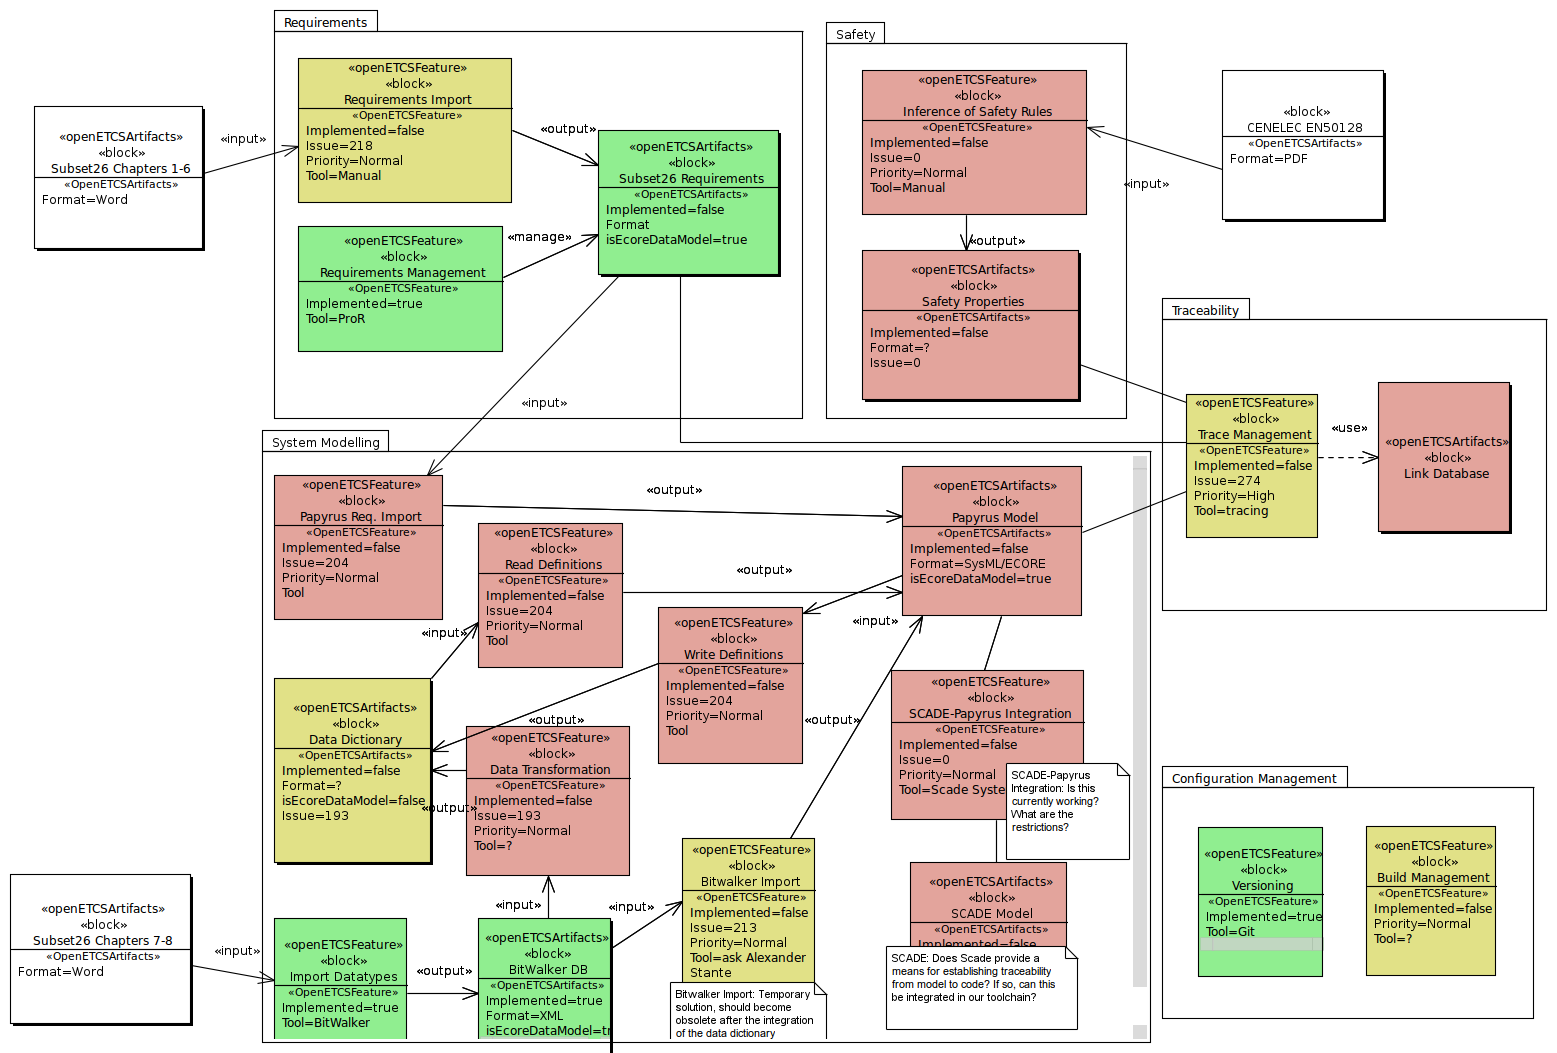
\includegraphics[width=\textwidth]{ToolChainmodel}
\caption{\label{fig:overview} Tool Chain overview (20.02.14) -- \\
  Green Block: Implemented \\
  Yellow Block: Work in Progress \\
  Red Block: Not started \\
  White Block: External Artifacts} 
\end{figure}
The features may be implemented by one or more tools and may also be implemented as plugins.
Currently, openETCS tool chain consists of the following components:
\begin{itemize}
\item Eclipse Kepler
\item Eclipse Modeling Tools
\item \href{http://www.eclipse.org/papyrus/}{[Eclipse Papyrus]}  
\item \href{http://eclipse.org/rmf/}{[Eclipse RMF]}
\item \href{http://www.eclipse.org/egit/}{[Eclipse EGit]}
\item \href{https://github.com/openETCS/toolchain/wiki/User-Documentation#Generating_Documentation}{[openETCS documentation Plugin]}
\item \href{https://github.com/openETCS/toolchain/wiki/Data-Dictionary-Plugin}{[openETCS DataDictionary Plugin]} 
\item \href{https://github.com/openETCS/toolchain/wiki/User-Documentation#Tracing_Requirements_and_SysML_Models}{[openETCS tracing Plugin]} 
\end{itemize}

\begin{center}
\begin{longtable}[H]{|p{6cm}|p{4cm}|p{4cm}|}\hline
\textbf{Test Items} & \textbf{Type of Test} & \textbf{Person in charge}\\\hline
\multirow{4}{*}{openETCS documentation Plugin} & Unit Testing & \\\cline{2-3} & Integration Testing & \\\cline{2-3} & Functional Testing & \\\cline{2-3} & Acceptance Testing & \\\hline
\multirow{4}{*}{openETCS DataDictionary Plugin} & Unit Testing & \\\cline{2-3} & Integration Testing & \\\cline{2-3} & Functional Testing & \\\cline{2-3} & Acceptance Testing & \\\hline
\multirow{4}{*}{openETCS tracing Plugin} & Unit Testing & \\\cline{2-3} & Integration Testing & \\\cline{2-3} & Functional Testing & \\\cline{2-3} & Acceptance Testing & \\\hline
\end{longtable}
\end{center}

\section{Features to be tested}
\label{sec:features_test}

\begin{center}
\begin{longtable}[H]{|p{2cm}|p{8cm}|}\hline
%\centering
%\begin{tabular}{|p{2cm}|p{8cm}|}\hline
\multicolumn{2}{|c|}{ProR}\\\hline
1 & Check if the RMF documentation is on Eclipse Help\\\hline
2 & Check if is possible to import a ProR requirements model\\\hline
3 & Check if it is possible to import a SysML requirements model\\\hline
4 & Check if it is possible to create a link between ProR and SysML\\\hline
5 & Check if it is possible to add extended attributes to the created links\\\hline
6 & Check how are created the required type of data.\\\hline
7 & Check if it is possible to delete required type of data\\\hline
8 & Check the plugin configuration\\ \hline
9 & ... \\ \hline
\multicolumn{2}{|c|}{Documentation}\\\hline
1 & Check if the documentation is on the eclipse help\\\hline
2 & Check if the links are correct in Eclipse Help\\\hline
3 & Check if the links are correct in the github wiki pages\\\hline
4 & Check if the links are correct in the PDF file\\\hline
5 & ...\\ \hline
\multicolumn{2}{|c|}{Data Dictionary}\\\hline
1 & \\ \hline
%\end{tabular}
\end{longtable}
\end{center}


\section{Item Pass / Fail Criteria}
A test is considered passed when the results obtained are the expected results shown in the Test Case. If any of the expected results are not met, the test is considered failed.

\section{Test Environment}
The environments where is going to be tested the toolchain are based on different operating systems:
\begin{itemize}
\item Windows 64
\item Windows 32
\item Linux 64
\item Linux 32
\item MacOS 64
\item MacOS 32
\end{itemize}

To perform the testing activities of the toolchain the following tools will be used:

\begin{center}
\begin{longtable}{|p{2cm}|p{8cm}|}\hline
\textbf{Tool} & \textbf{Functionality}\\\hline
GitHub & Configuration Management tool. This tool will be used to maintain under control all the selected configuration items (code, documentation,...), their versions and historial.\\\hline
Issue Tracker & Tool for the Bug Management and Tracking. The errors found during testing activities will be reported in this tool\\\hline
Jenkis & Open source continuous integration tool. This tool will be used to execute Unit tests.\\\hline
Maven &  Build automation tool. This tool will be used to execute some integration tests.\\\hline
Eclipse & Eclipse is a development tool and will be used for test, in functional testing, in an easy and agile way the Open ETCS pluggins.\\\hline
\end{longtable}
\end{center}

\begin{figure}[htbp]
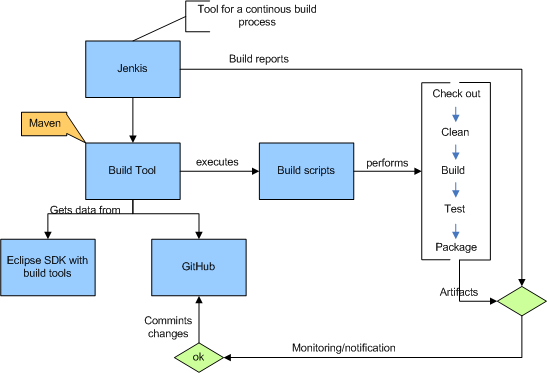
\includegraphics[width=\textwidth]{tools}
\caption{\label{fig:tools} Test environment tools} 
\end{figure}

\section{Test Deliverables}
Throughout the tool chain testing process a set of documents is created in order to keep track of the activities:
\begin{itemize}
\item \textbf{Test Plans}: A master test plan and sub-test plans for each plugin or feature will be developed. These documents will contain information about the scope, approach, objectives, features to be tested, resources, tools and schedule of testing activities.  These documents must be prepared in accordance with the EN50128 Standard. A Test Plan Template is provided in Appendices \ref{ref:test_plan_template}
\item \textbf{Test Specifications}: This document will contain all the information about the tests. For each of them, the ID, name, description and the requirements which the cases validate will be included. In addition, each Test Case will include information about the Entry and Exit specification, a Description of the Event to be performed and other information such as type or Needs Test Environment for conducting the test. The Test Specification Template is provided in the Appendices \ref{ref:test_spec_template}
\item \textbf{Test Results Reports}: The results obtained after the Test Cases execution will be collected in a Summary Test Report. For each test performed their unique identifier, the date and time which has been successfully executed or not and whether it is passed or failed state shall be indicated. A Test Results Report Template is provided in the Apendices \ref{ref:test_result_template}. In case the tests are executed automatically by a tool that creates its own report, this will also be used as Test Result Report. An example of this last condition is the unit test result report which can be found in \href{https://openetcs.ci.cloudbees.com/job/openETCS-tycho/lastBuild/testReport/}{[Test Report folder]}.
\item \textbf{Test Data}: All necessary data identified for use in test shoud be under configuration management tool.
\item \textbf{Test Incident Report}: This document will contain the list of errors found during the execution on test cases. For each error will appear the record of the ticket live.  
\item \textbf{Test Logs}: This document will contain the logs of the system during the OpenETCS platform testing.
\end{itemize}

\section{Schedule}
The plan of tasks related to the activities of the toolchain tests is detailed below:
\begin{center}
\begin{longtable}[H]{|p{8cm}|p{3cm}|p{3cm}|}\hline
\textbf{Activity} & \textbf{Start Date} & \textbf{End Date}\\\hline
Test Plan Elaboration & 14/08/2014 & 19/09/2014 \\\hline
Test Plan Review & 24/09/2014 & 26/09/2014\\\hline
Test Plan Corrections & 29/09/2014 & 30/09/2014\\\hline
Test Plan Approval & 01/10/2014 & 01/10/2014\\\hline
\multicolumn{3}{|l|}{Test Cases Specifications}\\\hline
Documentation Plugin Test Cases Specifications & 29/09/2014 & 02/10/2014\\\hline
Tracing Plugin Test Cases Specifications & & \\\hline
Data Dictionary Plugin Test Cases Specifications & & \\\hline
\multicolumn{3}{|l|}{Test Cases Review}\\\hline
Documentation Plugin Test Cases Review & & \\\hline
Tracing Plugin Test Cases Review & & \\\hline
Data Dictionary Plugin Test Cases Review & & \\\hline
\multicolumn{3}{|l|}{Test Cases Execution}\\\hline
Documentation Plugin Test Cases Execution & & \\\hline
Tracing Plugin Test Cases Execution & & \\\hline
Documentation Plugin Test Cases Execution & & \\\hline
\multicolumn{3}{|l|}{Test Results Report}\\\hline
Documentation Plugin Test Results Report & & \\\hline
Tracing Plugin Test Results Report & & \\\hline
Data Dictionary Plugin Test Results Report & & \\\hline
Regression testing & & \\\hline
\end{longtable}
\end{center}

\section{Responsabilities}
\begin{center}
\begin{longtable}[H]{|p{3cm}|p{8cm}|p{4cm}|}\hline
\textbf{Role} & \textbf{Responsabilities} & \textbf{Person in charge}\\\hline
WP7 Leader & \begin{itemize}
\item Review and approval of the toolchain testing strategy, approach, and plans
\item Review of testing results report and defects to determine the impact to overall tool chain and plugins  development and implementation schedule
\end{itemize}  
 & Michael Jastram\\\hline
Testing Manager & \begin{itemize}
\item Develop Test Strategy and Test Plan
\item Coordinate the development of testing deliverables
\item Review and approve testing deliverables
\item Monitor and report on the status of testing activities
\item Coordinate testing activities
\item Defect management
\end{itemize}  
 & \\\hline
SW Development Team & \begin{itemize}
\item Design Unit Test Cases
\item Execute Unit Test Cases
\item Review test cases and results for completeness
\end{itemize}  & Plugin or Feature Owner\\\hline
Tool chain Validation and Verification Team & \begin{itemize}
\item Design Test Cases
\item Execute Test Cases
\item Elaborate Test Reports
\end{itemize}
& \\\hline
\end{longtable}
\end{center}

\newpage
\begin{appendices}
   \addappheadtotoc
   \appendixpage

\section{Test Plan Template}
\label{ref:test_plan_template}

\subsection{Introduction}
\subsubsection{Executive Summary}
\subsubsection{Intended Audience}
\textit{This section of the Test Plan should list the audience for which the document has been written. Also mention distribution restrictions and levels of confidentiality}
\subsubsection{Evolution}
\subsubsection{References, Guidelines and Standards}
\textit{Provide a complete list of all documents and other sources referenced in the Software Test Plan}
\subsubsection{Definitions and Abbreviations}
\textit{Specify definitions of all terms and acronyms required to properly interpret the Test Results Report}

\subsection{Toolchain/Plugin Test Plan}
\subsubsection{Test Approach}
\textit{Identify the types of testing to be performed along with the methods and criteria to be used in performing test activities. Describe the specific methods and procedures for each type of testing.}
\subsubsection{Test Items}
\textit{Describe the items/features to be tested that are within the scope of the test plan}
\subsubsection{Features to be Tested}
\textit{Identify all toolchain features and combinations of features to be tested}
\subsubsection{Item Pass / Fail Criteria}
\textit{Specify the criteria to be used to determine whether each item has passed or failed testing}
\subsubsection{Test Environment}
\textit{Describe the tools and high level environment used for the testing activities}
\subsubsection{Test Deliverables}
\textit{Identify the deliverable documents from the test process}
\subsubsection{Schedule}
\textit{Identify the high level schedule for each testing task. Establish specific milestones for initiating and completing each type of test activity. Summarize when the testing activities will be done}
\subsubsection{Responsabilities}
\textit{Identify the groups responsible for managing, designing, preparing, executing, witnessing, checking, and resolving test activities}

\newpage
\section{Test Specification Template}
\label{ref:test_spec_template}
\begin{center}
\begin{longtable}{|p{3cm}|p{8cm}|}\hline
\multicolumn{2}{|c|}{\textbf{Test Case Identifier}: }\\\hline
Test Objective & \textit{Describe the purpose of the test case. Provide a brief description}\\\hline
Test Items & \textit{Describe the items or features (e.g., requirements, code, ...) to be tested by the test case}\\\hline
Input Specifications & \textit{Identify all inputs required to execute the test case.}\\\hline
Test Steps &  \textit{Describe the series of individually numbered steps that are to be completed in sequential order to execute the test.}\\\hline
Expected Test Results (Output Specifications) & \textit{Identify all outputs required to verify the test case. Describe what the system should look like after the test case is run.}\\\hline
Environmental needs &  \textit{Identify any environment requirement (e.g. operating system, tools,  }\\\hline
Inter-case Dependencies &  \textit{List any prerequisite test cases that would create the test environment or input data in order to run this test case.  Also, list any post-requisite test cases for which the running of this test case would create the test environment or input data.}\\\hline
\end{longtable}
\end{center}

\newpage
\section{Test Results Template}
\label{ref:test_result_template}

\subsection{Introduction}
\subsubsection{Purpose}
\textit{Provide the purpose of the Test Result Document}
\subsubsection{Audience}
\textit{This section of the Test Results Report should list the audience for which the document has been written. Also mention distribution restrictions and levels of confidentiality}
\subsubsection{References}
\textit{Provide a complete list of all documents and other sources referenced in the Software Test Plan}
\subsubsection{Definitions and Abbreviations}
\textit{Specify definitions of all terms and acronyms required to properly interpret the Test Results Report}

\subsection{Toolchain or plugins Test Summary}
\subsubsection{Objectives, Scope}
\textit{In the next section the objectives of the testing activities of the specific iteration are explained}
\subsubsection{Methodology}
\textit{In this section in which way the toolchain, and plugins requirements or features have been proven, the technique and tools that have been used, etc. will be explained}
\subsubsection{Results}
\textit{This section provides a summary of the results of the specific iteration testing of the toolchain and identifies all resolved issues. A list of requirements, test cases and the state, if passed or failed, will be created. In failed case the error number reported shall be identified}

\begin{center}
\begin{longtable}{|p{3cm}|p{2cm}|p{3cm}|p{3cm}|p{2cm}|}\hline
Test Identifier & State & Release version & Execution Date & Requirement covered Identifier\\\hline
 & & & & \\\hline
 & & & & \\\hline
\end{longtable}
\end{center}
\subsubsection{Evaluation}
\textit{This section provides an overall evaluation of the testing process}
\end{appendices}
